  \begin{center}
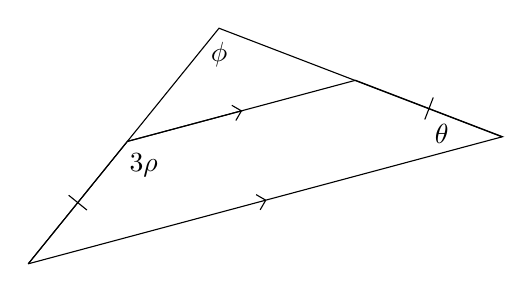
\begin{tikzpicture}[rotate=15]
\draw(0,0)--(36:2)--++(3,0)--++(-36:2)--++(-.8,0)node[anchor=south]{$\theta\degree$}--(0,0);
\draw(0,0)++(36:2)++(-.1,0)node[anchor=north west]{$3\rho\degree$};
\draw(0,0)++(36:2)--++(1.5,0)--++(-.1,.1)++(.1,-.1)--++(-.1,-.1);
\draw(0,0)--(36:3.85)node[anchor=north]{\rule{0mm}{3mm}$\phi\degree$}--++(-36:3.85);
\draw(36:1)--++(126:.15)--++(-54:.3);
\draw(0,0)++(36:2)++(3,0)++(-36:1)--++(54:.15)--++(-126:.3);
\draw(0,0)++(36:1.93)++(-36:1.93)--++(-.1,.1)++(.1,-.1)--++(-.1,-.1);
\end{tikzpicture}\\
Note: diagram is NOT to scale.
\end{center}
If $\phi=\theta$, what is the value of $\rho$?\\ \\


\ifsat
	\begin{enumerate}[label=\Alph*)]
	\end{enumerate}
\else
\fi

\ifacteven
	\begin{enumerate}[label=\textbf{\Alph*.},itemsep=\fill,align=left]
	\end{enumerate}
\else
\fi

\ifactodd
	\begin{enumerate}[label=\textbf{\Alph*.},itemsep=\fill,align=left]
	\end{enumerate}
\else
\fi

\ifgridin
$40$
\else
\fi

